

\subsection{Packet Loss Analysis}
Apart from studying the data usage volume, we also examine the packet loss data under the effect of COVID-19. As people were showing increased Internet usage during the lockdown period, potential network congestion might happen and can be reflected on the Internet packet loss rate. To quantify the packet loss rate, we define the metric as:

\begin{equation}
    Packet \ loss \% = \frac{\#Failure }{\#Failure + \#Success} \times 100
\end{equation}
Notice here we calculate using the 95\% quantile of the failure or success number at each time rather than the average value, because we are more interested in studying the packet loss change from top users. And we again shift the time to user's timezone locally.

\subsubsection{Daily Packet Loss}


\begin{figure}[ht]
\centering
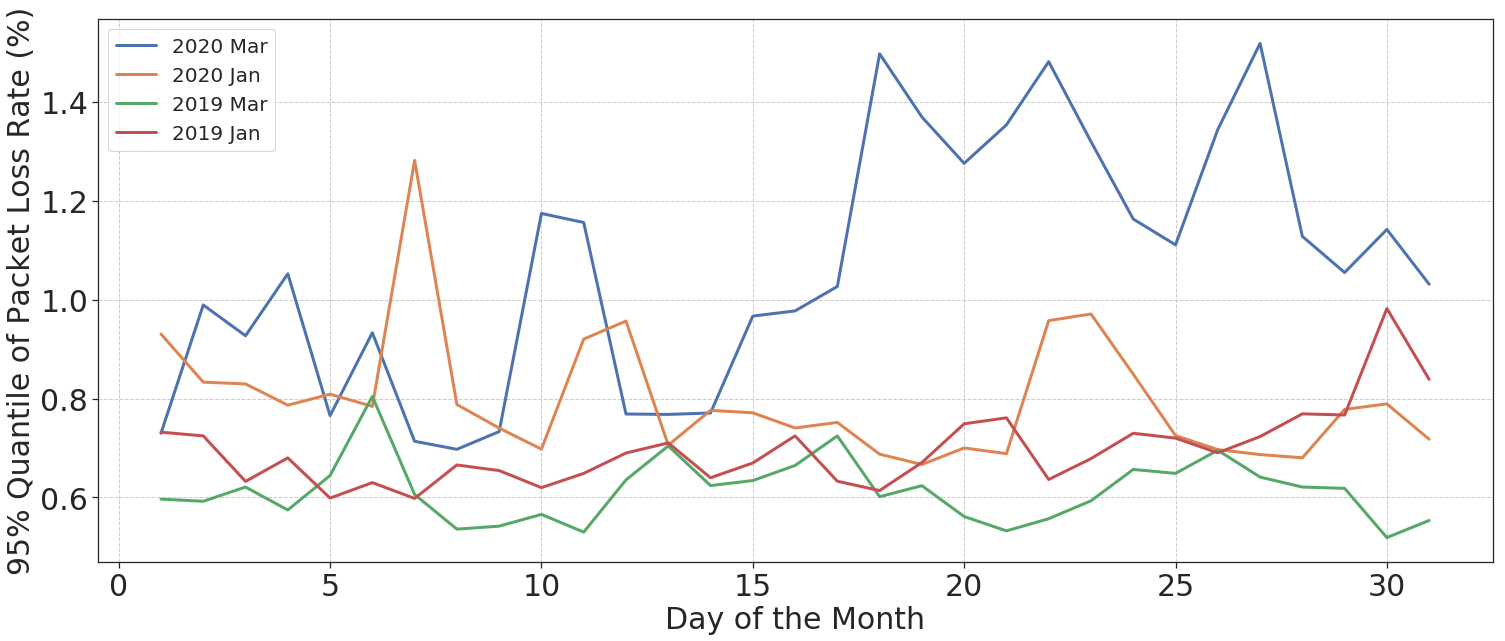
\includegraphics[width=1.0\linewidth]{figs/packet_loss_per_day.png}
\caption{Graph comparing the 95\% quantile packet loss per day for the month January, March 2019 and January, March 2020.}
\label{fig:packetlossperday}
\end{figure}
  
We found an significant increase in packet loss starting from mid-March 2020 (Figure \ref{fig:packetlossperday}), the period when some states initiated lockdown policy. The growth of this packet loss rate showed more than 40-50\% compared to that of early March, which is before the pandemic. On late March 2020, packet loss percentage could be 80\% higher than that before the pandemic, implying that large traffic congestion might occur. Since we do not observe similar trend from the same month in 2019, this impact may not occasionally result from the periodically change noise, but 
are caused by people's increasing Internet usage such as remote study, work from home and other online entertainment activities. 

However, by the end of March, the loss rate again started to decrease compared to the highest level. We speculate that the rapid response of the network operations help adjust the network capacity to the increasing need.

\subsubsection{Hourly Packet Loss}

\begin{figure}[ht]
\centering
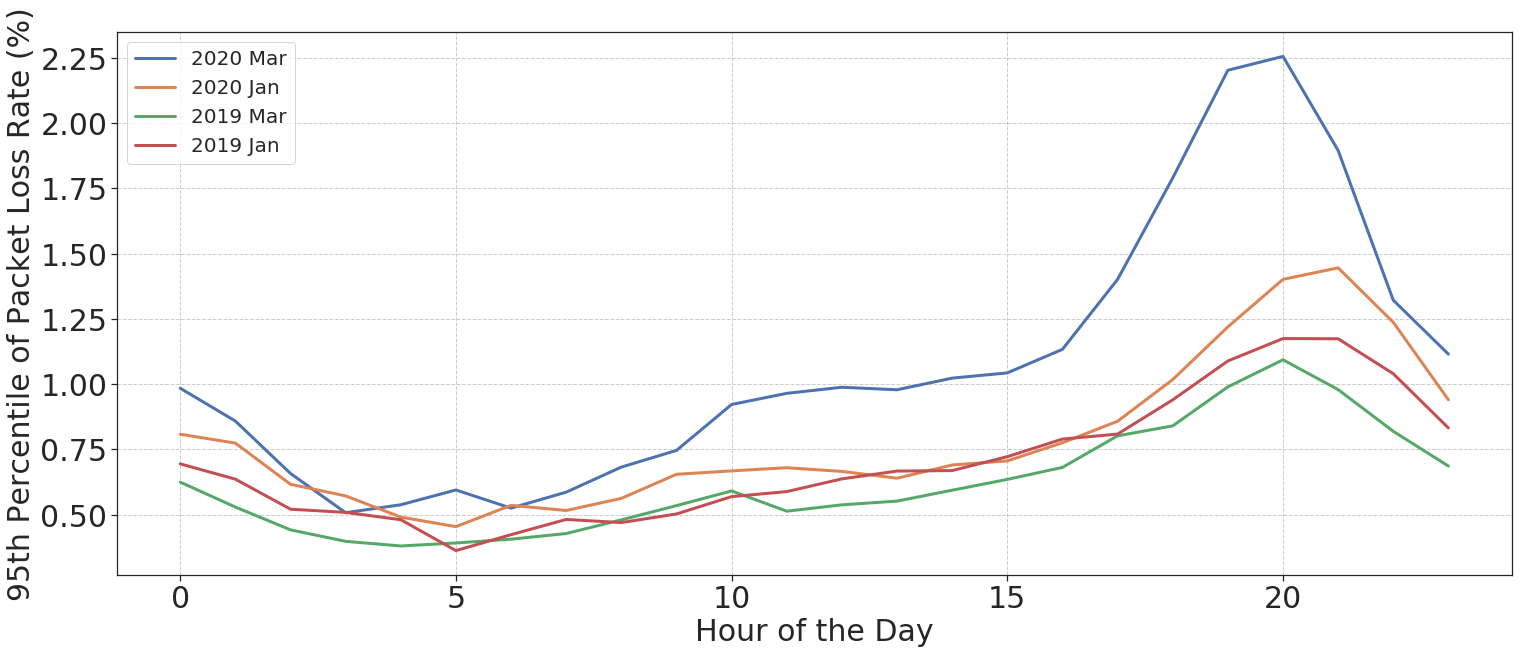
\includegraphics[width=1.0\linewidth]{figs/packet_loss_per_hour.png}
\caption{Graph comparing the 95\% quantile packet loss per hour for the month January, March 2019 and January, March 2020.}
\label{fig:packetlossperhour}
\end{figure}


When considering the effect of the time of the day, we found this packet loss change showed some interesting hourly pattern as well, which again might be related to people's online activities.

As we discussed in the diurnal data section above, the hourly packet loss rate showed similar trend due to the diurnal patterns of users’ Internet behavior (Figure \ref{fig:packetlossperhour}). In March 2020, the packet loss rate increased steeply in the daytime from 7:00 to 22:00, potentially due to the users' growing online activities like remote learning, work from home, etc. However, this change was more evident during the evening. For example, we saw an around 59\% growth from 18:00 to 22:00 when comparing March to January 2020. This difference suggests that packet loss is more positively related to the increased traffic due to recreational activities rather than remote working or distance learning. 


Our results are consistent with Candela et al. \cite{Candela2020latency}, as they found the increase of packet loss might be affected by factors like the type of target (whether belonging to a content delivery network or not), and the version of the Internet Protocol, and the time of the day as well.




%\subsubsection{95\% Hourly Packet Loss}
%Besides, we notice the same slight increase of capacity loss through the hourly packet loss data.
